\documentclass[11pt]{article}
\usepackage[margin=1.0in]{geometry}
\usepackage{amsmath,amssymb}
\usepackage{booktabs}
\usepackage{graphicx}
\usepackage{setspace}
\usepackage{xcolor}
\usepackage{titlesec}
\usepackage{placeins}
\usepackage{caption}
\captionsetup{font=small,labelfont=bf}
\usepackage[colorlinks=true,linkcolor=blue!60!black,citecolor=blue!60!black,urlcolor=blue!60!black]{hyperref}
\hypersetup{
    pdftitle={Ethnic Enclaves, Household Crowding, and Post-2020 Gateway Out-Migration: A Re-Examination (1980-2024)},
    pdfauthor={Daksh Tyagi and Gemini 4 Neon}
}
\emergencystretch=1.5em

\setstretch{1.14}
\titleformat{\section}{\normalfont\large\bfseries}{\thesection.}{0.6em}{}
\titleformat{\subsection}{\normalfont\normalsize\bfseries}{\thesubsection.}{0.5em}{}
\titlespacing*{\section}{0pt}{1.3em plus 0.3em minus 0.2em}{0.5em plus 0.1em}
\titlespacing*{\subsection}{0pt}{1.0em plus 0.2em minus 0.1em}{0.35em plus 0.1em}

\renewcommand{\topfraction}{0.85}
\renewcommand{\bottomfraction}{0.80}
\renewcommand{\textfraction}{0.12}
\renewcommand{\floatpagefraction}{0.95}
\setcounter{topnumber}{2}
\setcounter{bottomnumber}{1}
\setcounter{totalnumber}{2}

\begin{document}

\begin{center}
  \vspace*{0.2em}
  {\large\bfseries Ethnic Enclaves, Household Crowding, and Post-2020 Gateway\\[0.2em] Out-Migration: A Re-Examination (1980--2024)}\\[1.1em]
  {\normalsize\scshape Daksh Tyagi}\\[0.25em]
  {\normalsize\scshape Gemini 4 Neon}\\[0.5em]
  {\small\color{black!65} November 2026}
\end{center}
\vspace{0.9em}

\begin{list}{}{%
  \setlength{\leftmargin}{0.45in}%
  \setlength{\rightmargin}{0.45in}%
  \setlength{\parsep}{0pt}%
  \setlength{\topsep}{0pt}%
  \setlength{\itemsep}{0pt}%
  \setlength{\listparindent}{1.5em}%
}
\item\relax
\small\setstretch{1.11}%
\noindent\textsc{Abstract.} Why do U.S.-born descendants of immigrants remain in ethnic enclaves when immigration raises metropolitan housing costs? Using $17.71$ million harmonized Census and American Community Survey (ACS) observations from 1980 to 2024 linked to FHFA, Zillow, and O*NET data, we re-examine Song and Xu (2020) and Song (2017) across intra-metro housing adjustment, post-2020 gateway mobility, and shift-share instrumental-variables (IV) identification. Within-metro panels of unique households show no statistically significant rent or home-value discount with immigrant share even when endogenous room-count controls are excluded; instead, neighborhood crowding and three-or-more-generation households rise, U.S.-born co-ethnic adults experience higher crowding ($t = 2.20$), and common-sample dynamic-panel checks confirm severe downward Nickell bias in lagged-level price regressions. In the post-2020 period, descriptive gateway-exit regressions by current occupational teleworkability reflect only a transitory 2021 spike ($+0.53$ percentage points), while Webb wild cluster bootstrap inference across inter-metro movers finds no consistent positive differential in Sunbelt relocation or high-enclave arbitrage among observed gateway leavers amid wide uncertainty across eight origin clusters. Finally, exact closed-form Anderson--Rubin confidence sets confirm tightly bounded positive out-of-state-born adult clustering under static Bartik IV in both uniform decadal (1980--2010) and modern ACS (2010--2024) panels, whereas retention and static wage IVs lose first-stage power and yield unbounded confidence sets. This research was directed by Daksh Tyagi and carried out by a swarm of Gemini 4 Neon agents.

\vspace{0.6em}
\noindent{\footnotesize\color{black!70}\textbf{JEL Classification:} J15, J61, R21, R23, R31. \quad \textbf{Keywords:} Ethnic Enclaves, Household Crowding, Nickell Bias, Post-2020 Migration, Wild Cluster Bootstrap, Shift-Share IV.}
\end{list}

\vspace{1.0em}
\section{Introduction}

Why do U.S.-born descendants of immigrants remain clustered in ethnic enclaves when metropolitan immigration inflows raise citywide housing costs without clear local wage gains? Labor and urban economists have long debated how native-born populations respond to immigrant inflows (Card 2001, 2009; Borjas 2003, 2006; Peri and Sparber 2011; Card and Peri 2016). In the published benchmark for this literature, Song and Xu (2020) showed that ethnicity-specific immigrant inflows raise co-ethnic natives' local population share through higher retention and in-migration, pointing to sociocultural amenities rather than local labor-market returns; Song (2017, Ch.\ 3) further explored whether lower housing prices in immigrant-dense neighborhoods might offset rising citywide rents.

That housing-offset hypothesis sits in tension with two classic findings in urban economics. At the metropolitan scale, Saiz (2003, 2007) showed that immigration inflows push citywide rents and home values upward by raising aggregate housing demand. Inside metropolitan areas, Saiz and Wachter (2011) used a tract-level geographic-diffusion instrument to show that rapidly growing immigrant neighborhoods experienced \emph{slower} relative house-value appreciation alongside native flight, driven by socioeconomic and racial sorting. Evaluating housing adjustment inside cities therefore requires separating metropolitan demand shocks from neighborhood sorting, distinguishing household-level stock outcomes from person-level co-ethnic adult housing experience, omitting endogenous room-count controls when crowding is itself an adjustment margin, and auditing short-panel dynamic price regressions for mechanical Nickell (1981) bias.

The post-2020 expansion of remote work (Dingel and Neiman 2020; Barrero, Bloom, and Davis 2021; Ramani and Bloom 2021) offers a complementary descriptive lens on enclave location choices because historic immigrant gateways---New York, Los Angeles, San Francisco, Chicago, Miami, Washington DC, Boston, and Seattle---carry the highest housing costs in the United States. Measuring remote-work exposure in the ACS requires two safeguards: current occupation is recorded \emph{after} any one-year residential move and is therefore not pre-determined, and gateway-exit regressions contain only eight origin clusters, so asymptotic cluster-robust inference over-rejects without wild cluster bootstrap tests (Cameron, Gelbach, and Miller 2008; Webb 2023).

We assemble $17.71$ million harmonized U.S.\ Census and ACS working-age metropolitan observations from 1980 through 2024 (Ruggles et al.\ 2026) linked to FHFA (2026) and Zillow Research (2026) housing indices and O*NET task ratings (National Center for O*NET Development 2026), yielding three empirical findings.

On intra-metro housing adjustment, static within-metro OLS regressions on unique households across consistent sub-metro panels (2007--2024) show no statistically significant decline in neighborhood rents or home values with immigrant share, even when endogenous room and bedroom counts are omitted (Figure~\ref{fig:cpuma}). Because Public Use Microdata Areas (PUMAs) aggregate over roughly one hundred thousand residents and introduce spatial attenuation bias, these flat OLS estimates do not contradict Saiz and Wachter's (2011) tract-level IV evidence of slower neighborhood appreciation. Instead, sub-metro housing absorption appears clearly in household crowding (persons per room) and three-or-more-generation households at the neighborhood level, and in higher crowding experienced by U.S.-born co-ethnic working-age adults ($t = 2.20$). Re-estimating Song's (2017, Table 7) lagged-level price specification on a common non-singleton cell sample confirms severe downward Nickell (1981) bias on implied autoregressive persistence ($\hat{\rho}_{\text{FE}} = -0.31$ versus Anderson--Hsiao $\hat{\rho}_{\text{AH}} = -0.003$ for rent; $-0.25$ versus $+0.063$ for home value).

On post-2020 mobility, descriptive regressions show that gateway out-migration by current occupational teleworkability rests on a single transitory 2021 spike ($+0.53$ percentage points) beside a noisy 2018 pre-period point, whereas pre-determined 2015--2019 origin-metro telework exposure predicts broader out-migration ($+0.057^{***}$) without any differential gateway or enclave-retention shift. Across $99{,}329$ inter-metro co-ethnic movers ($99{,}074$ in regression samples) evaluated with Webb (2023) six-point wild cluster bootstrap inference ($G = 8$) and a sensitivity grid of seven distinct cutoff configurations around the baseline, we find no consistent positive differential in Sunbelt relocation or high-enclave arbitrage among observed gateway leavers, while underscoring the wide uncertainty inherent in eight origin clusters.

On shift-share identification, a disciplined weak-IV audit of Song and Xu (2020) and Song (2017) separates the analysis (Jaeger, Ruist, and Stuhler 2018) into a uniform ten-year decadal panel (1980--2010) and a separate modern ACS extension (2010--2024), applying two-way clustered Sanderson--Windmeijer (2016) conditional $F$-tests and exact closed-form Anderson--Rubin (1949) confidence sets without finite grid clipping. Out-of-state-born adult clustering is positive and tightly bounded under static Bartik IV in both eras ($+0.0321^{***}$ decadal; $+0.0252^{***}$ ACS), whereas retention and static wage IVs lose first-stage power (SW $F < 1$) and yield unbounded Anderson--Rubin sets, and uniform decadal dynamic two-instrument sets widen to include zero.

\section{Data, Measurement, and O*NET Teleworkability}

\subsection{Harmonized IPUMS USA Microdata (1980--2024) and Housing Series}

Our dataset combines U.S.\ Decennial Census 5 percent microdata (1980, 1990, and 2000) with 1-year ACS microdata (2007, 2010, 2015, 2018, 2019, and 2021--2024) from IPUMS USA (Ruggles et al.\ 2026), totaling $17.71$ million working-age (18--64), non-school metropolitan observations across 1980--2024. We begin in 1980 to avoid the 1970--1980 Census break from parental birthplace to open-ended self-reported ancestry, which spans all native generations and is subject to selective ethnic attrition (Duncan and Trejo 2011a, 2011b, 2017).\footnote{In IPUMS USA, parental birthplace (\texttt{FBPL}, \texttt{MBPL}) was replaced in 1980 by open-ended ancestry (\texttt{ANCESTR1}, \texttt{ANCESTR2}). Metropolitan areas are harmonized to 2013 OMB boundaries (\texttt{MET2013}), foreign-born origins use birthplace (\texttt{BPL}), unique householders use \texttt{PERNUM}=1 weighted by \texttt{HHWT}, person-level regressions use \texttt{PERWT}, and strict three-or-more-generation households use \texttt{MULTGEN}=3 (excluding ordinary two-generation households, \texttt{MULTGEN}=2).}

Metropolitan areas are harmonized to consistent 2013 OMB boundaries across 35 major origin groups, linking foreign-born immigrants by country of birth to U.S.-born co-ethnics by ancestry. Weighting follows the exact unit of observation: household-level neighborhood housing outcomes (Section 3, Panels A and C) aggregate strictly over unique working-age householders weighted by household weights so multi-adult households are never multi-counted, whereas person-level co-ethnic adult housing experience (Section 3, Panel B), labor-market outcomes, and migration regressions use person weights. We define multigenerational living strictly as three-or-more-generation households, excluding ordinary two-generation parent--child households.

For sub-metro housing analysis, we exclude group quarters and separate the 2007--2021 consistent sub-metro panel ($4{,}564$ neighborhood-year cells; $105{,}646$ co-ethnic cells) from the 2022--2024 post-2020-Census PUMA panel ($5{,}607$ cells) to prevent boundary breaks.\footnote{Sub-metro panels use IPUMS \texttt{CPUMA0010} (2007--2021) and 2020-Census \texttt{PUMA} (2022--2024). Migration windows strictly separate 5-year Census moves (\texttt{MIGMETAREA5}, 1980--2000) from 1-year ACS moves (\texttt{MIGMET131}, 2010--2024).} For migration, we strictly separate 5-year Census migration windows (1980--2000) from 1-year ACS migration windows (2010--2024). Metropolitan housing benchmarks come from the FHFA House Price Index (1975--2026; FHFA 2026) and Zillow's Home Value Index (ZHVI, 2000--2026) and Observed Rent Index (ZORI, 2015--2026; Zillow Research 2026).

\subsection{O*NET 31.0 Teleworkability and Timing Caveat}

Following Dingel and Neiman (2020), we classify 911 O*NET 31.0 occupations across 41 Generalized Work Activities as non-teleworkable if any of nine physical, outdoor, equipment, repair, care, or public-contact tasks scores at least $4.0$ on Importance or if \emph{Working with Computers} scores below $3.0$, matching $660$ of $665$ ACS occupation codes.\footnote{Occupations are matched on IPUMS \texttt{OCCSOC}, and realized work-from-home is defined as \texttt{TRANWORK == 80}.} In the 2021--2024 ACS, $42.7$ percent of metropolitan employment falls in teleworkable occupations, and realized work-from-home reaches $26.6$ percent in teleworkable jobs versus $8.8$ percent in non-teleworkable jobs (cross-occupation $r = 0.760$ in levels; $r = 0.801$ in post-2020 changes).

A critical identification boundary governs ACS mobility analysis: the ACS records a respondent's \emph{current} occupation at the survey date, \emph{after} any one-year residential move. Because workers planning to relocate may switch occupations before or upon moving, individual occupational teleworkability is not pre-determined and cannot support causal intent-to-treat claims. We therefore label all individual-occupation regressions in Sections 4 and 5 as descriptive comparisons, and supplement Section 4 with a genuinely pre-determined 2015--2019 origin-metro (and origin-metro $\times$ ethnicity) telework exposure measure.

\section{Sub-Metro Housing Costs, Crowding, and Nickell Bias (1980--2024)}

\subsection{Within-Metro Specification, Unit of Observation, and Saiz--Wachter (2011)}

To examine how housing markets adjust inside metropolitan areas, we estimate static within-metro OLS regressions separately on the 2007--2021 consistent sub-metro panel and the 2022--2024 post-2020 PUMA panel:
\begin{equation}
Y_{pct} = \beta \cdot \text{ImmShare}_{pct} + X_{pct}'\Gamma + \alpha_{pc} + \rho_{ct} + \varepsilon_{pct},
\end{equation}
where $\rho_{ct}$ absorbs metropolitan-by-year shocks and $\alpha_{pc}$ absorbs neighborhood fixed effects, with standard errors clustered by metropolitan area. In Panels A and C of Table~\ref{tab:cpuma_housing}, $Y_{pct}$ averages housing outcomes across unique householders using household weights. In Panel B, $Y_{rpct}$ measures the average housing conditions \emph{experienced by U.S.-born co-ethnic working-age adults} using person weights, capturing co-ethnic adults in both own-headed and parent-headed households while absorbing ethnicity-by-year, metro-by-year, and ethnicity-by-neighborhood fixed effects.

Two methodological considerations require explicit care. When household crowding (persons per room) is itself an adjustment margin, controlling for unit room and bedroom counts introduces a bad-control problem because families facing tight housing markets endogenously choose smaller or more densely shared units.\footnote{Full Hedonic controls add mean \texttt{ROOMS} and \texttt{BEDROOMS}, whereas Structure-Only controls retain only pre-determined building attributes (\texttt{BUILTYR2} and \texttt{UNITSSTR}), homeownership share, mean age, and mean education.} We therefore report a parallel \emph{Structure-Only} specification controlling solely for pre-determined building attributes, homeownership share, mean age, and mean education alongside the full hedonic specification. In addition, these within-metro regressions are static OLS without a neighborhood-level instrument, and PUMAs ($\sim$100,000+ residents) aggregate over diverse census tracts, introducing classical spatial attenuation bias. Consequently, our PUMA-level estimates should not be read as overturning Saiz and Wachter (2011), who used a tract-level geographic-diffusion IV to document slower neighborhood house-value appreciation and native flight in rapidly growing immigrant tracts; rather, they test whether a systematic housing-price discount appears at the sub-metro scale and quantify crowding and three-or-more-generation living margins.

\subsection{Results: Flat Sub-Metro Prices, Crowding, and Common-Sample Nickell Bias}

Table~\ref{tab:cpuma_housing} and Figure~\ref{fig:cpuma} summarize the sub-metro housing, crowding, and dynamic-panel results. Across Panels A--C, omitting endogenous room and bedroom counts leaves every price estimate virtually unchanged. Among unique households in 2007--2021 consistent sub-metro neighborhoods ($N = 4{,}564$), log gross rent shows no statistically significant relationship with immigrant share under Structure-Only controls ($+0.00033$, SE $0.00048$, $t = +0.69$) or Full Hedonic controls ($+0.00018$, SE $0.00050$, $t = +0.36$); log home value is likewise flat ($+0.00048$, SE $0.00109$ Structure-Only; $+0.00014$, SE $0.00106$ Full Hedonic). U.S.-born co-ethnic adult housing costs in Panel B ($-0.00059$, SE $0.00135$ for rent; $-0.00198$, SE $0.00307$ for home value) show no detectable discount. Unique households in 2022--2024 PUMA neighborhoods in Panel C ($+0.00050$, SE $0.00044$ for rent; $-0.00012$, SE $0.00056$ for home value) are similarly flat at the PUMA scale, whereas metropolitan Zillow rents rise $+1.06\%^{***}$ per percentage-point inflow (Saiz 2003, 2007).

\begin{table}[t!]
\centering
\caption{Within-Metro Housing Prices, Crowding, 3+ Generation Living, and Dynamic-Panel Nickell (1981) Bias}
\label{tab:cpuma_housing}
\scriptsize
\setlength{\tabcolsep}{4.0pt}
\renewcommand{\arraystretch}{1.04}
\begin{tabular}{lccccc}
\toprule
Outcome Specification & Coef. & (SE) & $t$-stat & $N$ & FE / Implied $\hat{\rho}$ \\
\midrule
\multicolumn{6}{l}{\textit{Panel A: Within-MSA \texttt{CPUMA0010} Unique Households (\texttt{PERNUM}=1, \texttt{HHWT}-Weighted, 2007--2021)}} \\
Log Gross Rent (Unadjusted) & +0.0006 & (0.0006) & +1.06 & 4,564 & MSA$\times$Yr + CPUMA \\
Log Gross Rent (Structure-Only, No Rooms) & +0.0003 & (0.0005) & +0.69 & 4,564 & MSA$\times$Yr + CPUMA \\
Log Gross Rent (Full Hedonic) & +0.0002 & (0.0005) & +0.36 & 4,564 & MSA$\times$Yr + CPUMA \\
Log Home Value (Structure-Only, No Rooms) & +0.0005 & (0.0011) & +0.44 & 4,564 & MSA$\times$Yr + CPUMA \\
Log Home Value (Full Hedonic) & +0.0001 & (0.0011) & +0.13 & 4,564 & MSA$\times$Yr + CPUMA \\
Household Crowding (Persons/Room, All HHs) & +0.0021*** & (0.0002) & +8.52 & 4,564 & MSA$\times$Yr + CPUMA \\
3+ Generation Households (\texttt{MULTGEN}=3) & +0.0004*** & (0.0001) & +6.26 & 4,564 & MSA$\times$Yr + CPUMA \\
\midrule
\multicolumn{6}{l}{\textit{Panel B: U.S.-Born Co-Ethnic Adult Housing Experience in \texttt{CPUMA0010} (\texttt{PERWT}-Weighted, 2007--2021)}} \\
Co-Ethnic Adult Log Rent (Structure-Only) & -0.0006 & (0.0013) & -0.43 & 74,204 & 3-Way FE \\
Co-Ethnic Adult Log Rent (Full Hedonic) & -0.0013 & (0.0013) & -0.97 & 74,204 & 3-Way FE \\
Co-Ethnic Adult Log Value (Structure-Only) & -0.0020 & (0.0031) & -0.64 & 93,690 & 3-Way FE \\
Co-Ethnic Adult Crowding (Persons/Room) & +0.0028** & (0.0013) & +2.20 & 105,646 & 3-Way FE \\
Co-Ethnic Adult 3+ Gen Living (\texttt{MULTGEN}=3) & +0.0012 & (0.0008) & +1.51 & 105,646 & 3-Way FE \\
\midrule
\multicolumn{6}{l}{\textit{Panel C: Post-COVID 2020-Census \texttt{PUMA} Unique Households (\texttt{PERNUM}=1, \texttt{HHWT}-Weighted, 2022--2024)}} \\
Log Gross Rent (Structure-Only, No Rooms) & +0.0005 & (0.0004) & +1.14 & 5,607 & MSA$\times$Yr + PUMA \\
Log Home Value (Structure-Only, No Rooms) & -0.0001 & (0.0006) & -0.22 & 5,607 & MSA$\times$Yr + PUMA \\
Household Crowding (Persons/Room, All HHs) & +0.0021*** & (0.0003) & +7.50 & 5,607 & MSA$\times$Yr + PUMA \\
3+ Generation Households (\texttt{MULTGEN}=3) & +0.0004*** & (0.0001) & +3.10 & 5,607 & MSA$\times$Yr + PUMA \\
\midrule
\multicolumn{6}{l}{\textit{Panel D: Common-Sample Nickell (1981) Bias Check on Song's Table 7 (1980--2024 Cell Panel)}} \\
$\Delta \ln(\text{Rent})$: Dynamic FE ($hp_{t-1}$ + 3-Way FE) & +0.0047* & (0.0026) & +1.83 & 12,203 & $\hat{\rho}_{\mathrm{FE}}=-0.31$ ($\hat{\gamma}=-1.31$) \\
$\Delta \ln(\text{Rent})$: Static FD (No Lag, 3-Way FE) & +0.0013 & (0.0026) & +0.52 & 12,203 & No dynamic lag \\
$\Delta \ln(\text{Rent})$: Anderson--Hsiao IV ($hp_{t-2}$) & +0.0035* & (0.0020) & +1.70 & 12,203 & $\hat{\rho}_{\mathrm{AH}}=-0.00$ ($F_1=210$) \\
$\Delta \ln(\text{Value})$: Dynamic FE ($hp_{t-1}$ + 3-Way FE) & -0.0029 & (0.0038) & -0.74 & 14,525 & $\hat{\rho}_{\mathrm{FE}}=-0.25$ ($\hat{\gamma}=-1.25$) \\
$\Delta \ln(\text{Value})$: Static FD (No Lag, 3-Way FE) & -0.0090** & (0.0037) & -2.44 & 14,525 & No dynamic lag \\
$\Delta \ln(\text{Value})$: Anderson--Hsiao IV ($hp_{t-2}$) & -0.0049* & (0.0029) & -1.65 & 14,525 & $\hat{\rho}_{\mathrm{AH}}=+0.06$ ($F_1=538$) \\
\bottomrule
\end{tabular}
\begin{minipage}{0.96\linewidth}
\footnotesize\textit{Notes:} IPUMS ACS microdata (working-age 18--64, non-school, non-GQ), clustered by MSA. Panels A and C aggregate unique households (\texttt{PERNUM}=1, weighted by \texttt{HHWT}) and define three-or-more-generation households strictly as \texttt{MULTGEN}=3. Panel B averages housing conditions experienced by U.S.-born co-ethnic working-age adults using person weights (\texttt{PERWT}), absorbing Eth$\times$Yr, MSA$\times$Yr, and Eth$\times$CPUMA FEs. Structure-Only omits endogenous room/bedroom counts and controls only for \texttt{BUILTYR2}, \texttt{UNITSSTR}, homeownership, age, and education; Full Hedonic adds mean rooms and bedrooms. Panel D estimates $\Delta hp_{rct}$ on $\Delta \text{Share}_{rct}$ on the exact same non-singleton common cell sample with identical differenced controls ($\Delta\text{Educ}$, $\Delta\ln\text{Wage}$), comparing implied persistence $\hat{\rho}_{\text{FE}} = 1 + \hat{\gamma}$ under Dynamic FE against $\hat{\rho}_{\text{AH}}$ under Anderson--Hsiao IV. $^{***}p<0.01$, $^{**}p<0.05$, $^{*}p<0.10$.
\end{minipage}
\end{table}


By contrast, intensive-margin crowding and three-or-more-generation living rise consistently at the neighborhood level. Across unique households, crowding increases by $+0.00206^{***}$ persons per room ($t = +8.52$) in 2007--2021 and $+0.00211^{***}$ ($t = +7.50$) in 2022--2024, alongside higher three-or-more-generation household shares ($+0.00042^{***}$, $t = +6.26$ in 2007--2021; $+0.00041^{***}$, $t = +3.10$ in 2022--2024). Because all-household crowding partly reflects immigrant household composition, the cleaner test is U.S.-born co-ethnic working-age adults in Panel B ($N = 105{,}646$, person-weighted): co-ethnic adult crowding rises $+0.00283^{**}$ ($t = +2.20$) per percentage-point local co-ethnic immigrant share, while crowding among all native-headed households in the same neighborhood is negative ($-0.00065^{**}$, $t = -2.30$). Restricting multigenerational living strictly to three-or-more-generation households yields a positive but imprecisely estimated co-ethnic adult slope ($+0.00122$, SE $0.00081$, $t = +1.51$).

Panel D of Table~\ref{tab:cpuma_housing} provides an algebraically consistent empirical check of Nickell (1981) bias in Song's (2017, Table 7) lagged-level price specification. To ensure a valid comparison, all three estimators are run on the exact same non-singleton common cell sample ($N = 12{,}203$ for rent; $N = 14{,}525$ for house value) with identical differenced controls ($\Delta \text{Educ}$ and $\Delta \ln \text{Wage}$). In Song's dynamic fixed-effects equation $\Delta hp_{it} = \gamma hp_{i,t-1} + \beta \Delta \text{Share}_{it} + \dots + \alpha_i$, the coefficient $\gamma$ estimates $\rho-1$, so implied autoregressive persistence is $\hat{\rho}_{\text{FE}} = 1+\hat{\gamma}$, directly comparable to $\hat{\rho}_{\text{AH}}$ on $\Delta hp_{i,t-1}$ in Anderson and Hsiao (1981) IV (where first-differencing eliminates $\alpha_i$ and $hp_{i,t-2}$ instruments $\Delta hp_{i,t-1}$). For $\Delta \ln(\text{Rent})$, including $hp_{t-1}$ alongside ethnicity-by-MSA fixed effects yields $\hat{\gamma} = -1.3146$ (SE $0.0174$), implying sharp negative persistence $\hat{\rho}_{\text{FE}} = -0.3146$, whereas Anderson--Hsiao IV ($F_1 = 210.0$) recovers $\hat{\rho}_{\text{AH}} = -0.0027$ (SE $0.0260$), a downward Nickell bias of roughly $-0.31$ on $\rho$; the co-ethnic inflow coefficient shifts from $+0.00469^{*}$ (Dynamic FE) to $+0.00133$ (no-lag static FD) and $+0.00347^{*}$ (Anderson--Hsiao IV). For $\Delta \ln(\text{Value})$, Dynamic FE similarly yields $\hat{\rho}_{\text{FE}} = -0.2458$ ($\hat{\gamma} = -1.2458$, SE $0.0164$) versus Anderson--Hsiao $\hat{\rho}_{\text{AH}} = +0.0632$ (SE $0.0222$, $F_1 = 537.8$), shifting $\hat{\beta}$ from $-0.00286$ to $-0.00903^{**}$ (no lag) and $-0.00486^{*}$ (Anderson--Hsiao IV).

\begin{figure}[t!]
\centering
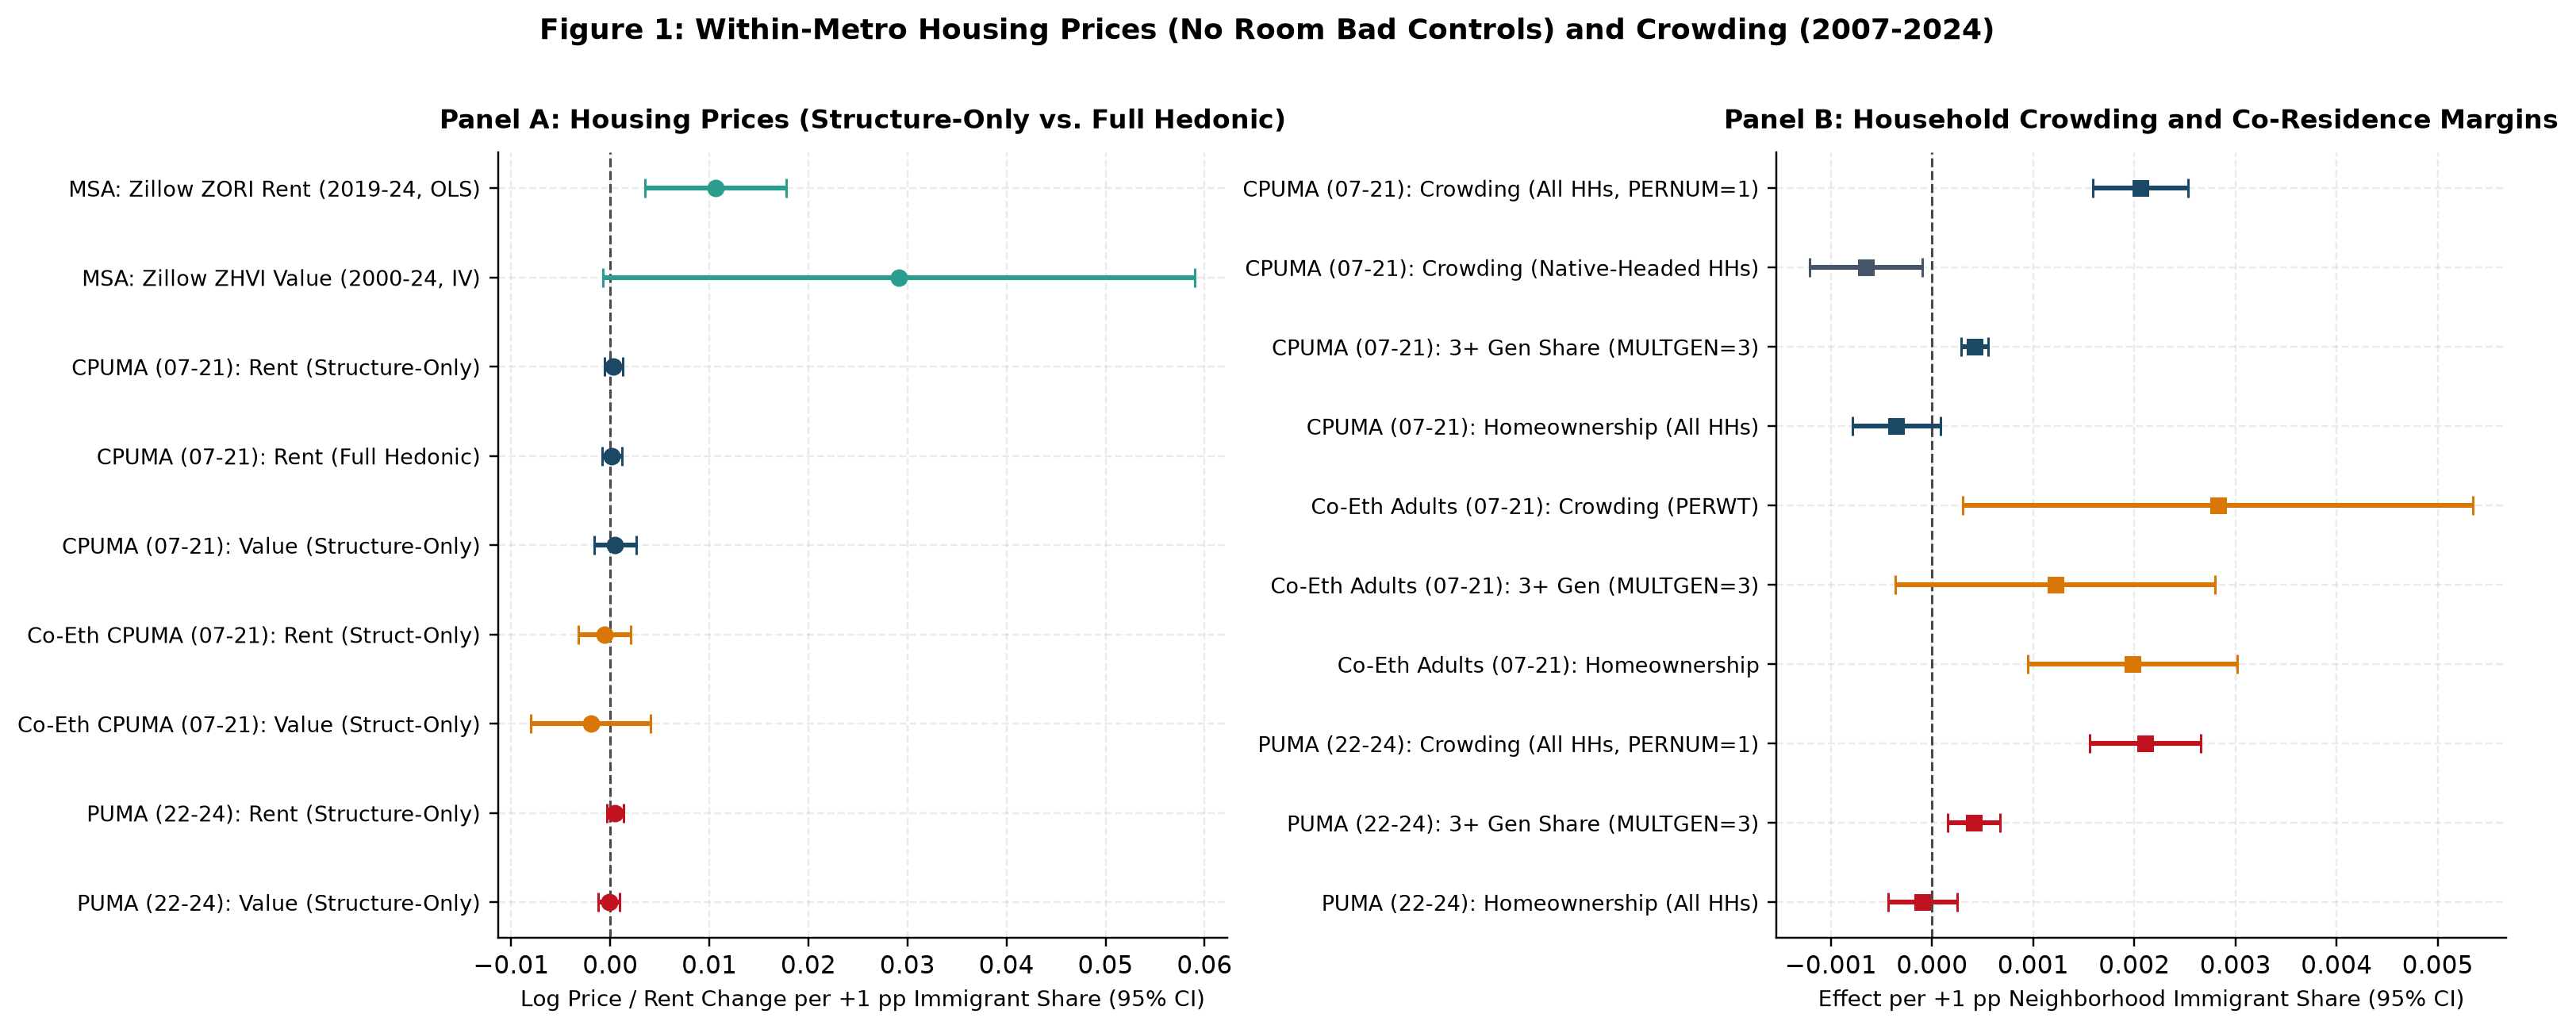
\includegraphics[width=0.90\linewidth,height=0.33\textheight,keepaspectratio]{figures/fig1_cpuma_neighborhood_vs_msa.png}
\caption{Within-Metro Housing Prices, Crowding, and Three-or-More-Generation Living, 2007--2024. \normalfont Panel~A compares metropolitan Zillow benchmarks against within-metro Structure-Only (no room or bedroom controls) and Full Hedonic specifications across 2007--2021 consistent sub-metro areas and 2022--2024 PUMAs. Panel~B separates unique householders (household-weighted) from U.S.-born co-ethnic adult housing experience (person-weighted; crowding $t = 2.20$) and strict three-or-more-generation households.}
\label{fig:cpuma}
\end{figure}

\section{Descriptive Post-2020 Mobility by Teleworkability and Pre-2019 Origin Exposure}

To examine whether post-2020 remote work reshaped gateway out-migration or enclave retention, we estimate descriptive triple-difference and event-study models over $3.31$ million U.S.-born co-ethnic adults in the 2015, 2018, 2019, and 2021--2024 ACS waves:
\begin{equation}
Y_{irct} = \sum_{\tau \ne 2019} \delta_\tau \cdot \mathbf{1}[t=\tau] \cdot \text{Tele}_i \cdot \text{Exp}_{rc,\text{pre}} + \text{Lower-Order} + X_{it}'\Gamma + \nu_{rt} + \rho_{ct} + \theta_{rc} + \lambda_{\text{tele},t} + u_{irct},
\end{equation}
absorbing ethnicity-by-year, metro-by-year, ethnicity-by-metro, and teleworkable-by-year fixed effects, with standard errors clustered by metropolitan area. Because $\text{Tele}_i$ is assigned from current occupation observed after any residential move, we treat Panel A of Table~\ref{tab:telework_did} as descriptive and pair it in Panel B with genuinely pre-determined 2015--2019 origin-metro and origin-metro $\times$ ethnicity teleworkable employment shares.

\begin{table}[t!]
\centering
\caption{Post-2020 Mobility, Wages, and Rent Burden by Occupational Teleworkability and Pre-2019 Origin-Metro Exposure (2015--2024)}
\label{tab:telework_did}
\scriptsize
\setlength{\tabcolsep}{3pt}
\renewcommand{\arraystretch}{1.05}
\begin{tabular}{llcccc}
\toprule
Outcome & Interaction Term & Coef. & (SE) & $t$-stat & Micro $N$ \\
\midrule
\multicolumn{6}{l}{\textit{Panel A: Descriptive Associations by Current Occupational Teleworkability (\texttt{OCCSOC})}} \\
Realized WFH (\texttt{TRANWORK}=80) & $\text{Tele} \times \text{Post2020}$ & +0.13508*** & (0.00383) & +35.27 & 3,309,606 \\
Gateway Out-Migration Rate & $\text{Tele} \times \text{Post} \times \text{Top8Gateway}$ & +0.00185** & (0.00091) & +2.03 & 3,309,606 \\
True Origin-MSA Retention & $\text{Tele} \times \text{Post} \times \text{PreEnclaveShare}$ & +0.00002 & (0.00007) & +0.24 & 3,309,606 \\
Within-Gateway Out-Migration & $\text{Tele} \times \text{Post} \times \text{PreEnclaveShare}$ & +0.00002 & (0.00014) & +0.12 & 828,063 \\
Log Real Hourly Wage & $\text{Tele} \times \text{Post} \times \text{PreEnclaveShare}$ & -0.00083* & (0.00044) & -1.89 & 3,365,602 \\
Rent Burden (Rent/Wage Income) & $\text{Tele} \times \text{Post} \times \text{PreEnclaveShare}$ & +0.00075** & (0.00031) & +2.41 & 3,249,988 \\
\midrule
\multicolumn{6}{l}{\textit{Panel B: Genuinely Pre-Determined Origin-Metro Pre-2019 Telework Exposure}} \\
All-MSA Out-Migration Rate & $\text{OrigMetroTele}_{15-19} \times \text{Post}$ & +0.05706*** & (0.01729) & +3.30 & 3,280,750 \\
Gateway Out-Migration (Metro Exp.) & $\text{OrigMetroTele}_{15-19} \times \text{Post} \times \text{GW}$ & +0.03307 & (0.05741) & +0.58 & 3,280,750 \\
Gateway Out-Migration (Eth-Metro Exp.) & $\text{OrigEthTele}_{15-19} \times \text{Post} \times \text{GW}$ & +0.00997 & (0.00984) & +1.01 & 3,280,750 \\
True Retention (Eth-Metro Exp.) & $\text{OrigEthTele}_{15-19} \times \text{Post} \times \text{Share}$ & -0.00106 & (0.00174) & -0.61 & 3,280,750 \\
\bottomrule
\end{tabular}
\begin{minipage}{0.96\linewidth}
\footnotesize\textit{Notes:} IPUMS ACS 2015, 2018, 2019 (Pre) vs.\ 2021--2024 (Post), U.S.-born co-ethnic working-age adults. Panel A classifies workers by current-year \texttt{OCCSOC} (observed after any 1-year move; hence descriptive, not causal), absorbing Eth$\times$Yr, MSA$\times$Yr, Eth$\times$MSA, and Tele$\times$Yr FEs. Panel B uses genuinely pre-determined 2015--2019 origin-metro (or origin-metro $\times$ ethnicity) teleworkable employment shares. SEs clustered by origin/destination MSA. $^{***}p<0.01$, $^{**}p<0.05$, $^{*}p<0.10$.
\end{minipage}
\end{table}


Table~\ref{tab:telework_did} and Figure~\ref{fig:event_study} reveal a far more modest and transitory pattern than headline remote-work narratives suggest. While workers in teleworkable occupations became $+13.51$ percentage points$^{***}$ ($t = 35.27$) more likely to work from home after 2020, the pooled post-2020 gateway-exit association ($+0.185$ pp, SE $0.091$ pp, $p = 0.043$) masks sharp year-by-year instability. In Panel A of Figure~\ref{fig:event_study}, the 2018 pre-period coefficient ($+0.25$ pp, SE $0.23$ pp, $p = 0.28$) is larger than the pooled post-2020 estimate ($+0.185$ pp), and the entire post-2020 shift consists of a single transitory 2021 spike ($+0.53$ pp, SE $0.16$ pp, $p = 0.001$) that reverted immediately in 2022 ($+0.11$ pp, $p = 0.56$) and 2023 ($+0.05$ pp, $p = 0.78$), with no statistically significant resurgence in 2024 ($+0.23$ pp, SE $0.15$ pp, $p = 0.14$).

Across all metropolitan areas, true one-year origin-MSA retention shows no post-2020 shift ($+0.00002$, SE $0.00007$, $p = 0.81$), sitting near zero in every event-study year (Panel B). For stayers in high-enclave metros, the pooled post-2020 rent-burden coefficient is positive ($+0.00075^{**}$, $p = 0.017$), yet every individual event-study year in Panel D is statistically insignificant ($p = 0.50$ in 2021, $p = 0.17$ in 2022, $p = 0.31$ in 2023, and $p = 0.31$ in 2024), providing too little precision to claim a sustained climb. Log hourly wages show a marginal pooled dip ($-0.00083^{*}$, $p = 0.059$), likewise insignificant in 2021--2023.

Panel B of Table~\ref{tab:telework_did} evaluates genuinely pre-determined 2015--2019 origin-metro telework exposure, which cannot be contaminated by post-move occupation switching. Metros with higher pre-2019 teleworkable employment shares experienced significantly higher overall post-2020 out-migration ($+0.05706^{***}$, SE $0.01729$, $p = 0.001$, consistent with Ramani and Bloom 2021). However, the incremental gateway interaction is statistically insignificant both at the metro level ($+0.03307$, SE $0.05741$, $p = 0.565$) and at the ethnicity-by-metro level with full three-way fixed effects ($+0.00997$, SE $0.00984$, $p = 0.312$), and origin-metro enclave retention remains null ($-0.00106$, $p = 0.541$).

\begin{figure}[t!]
\centering
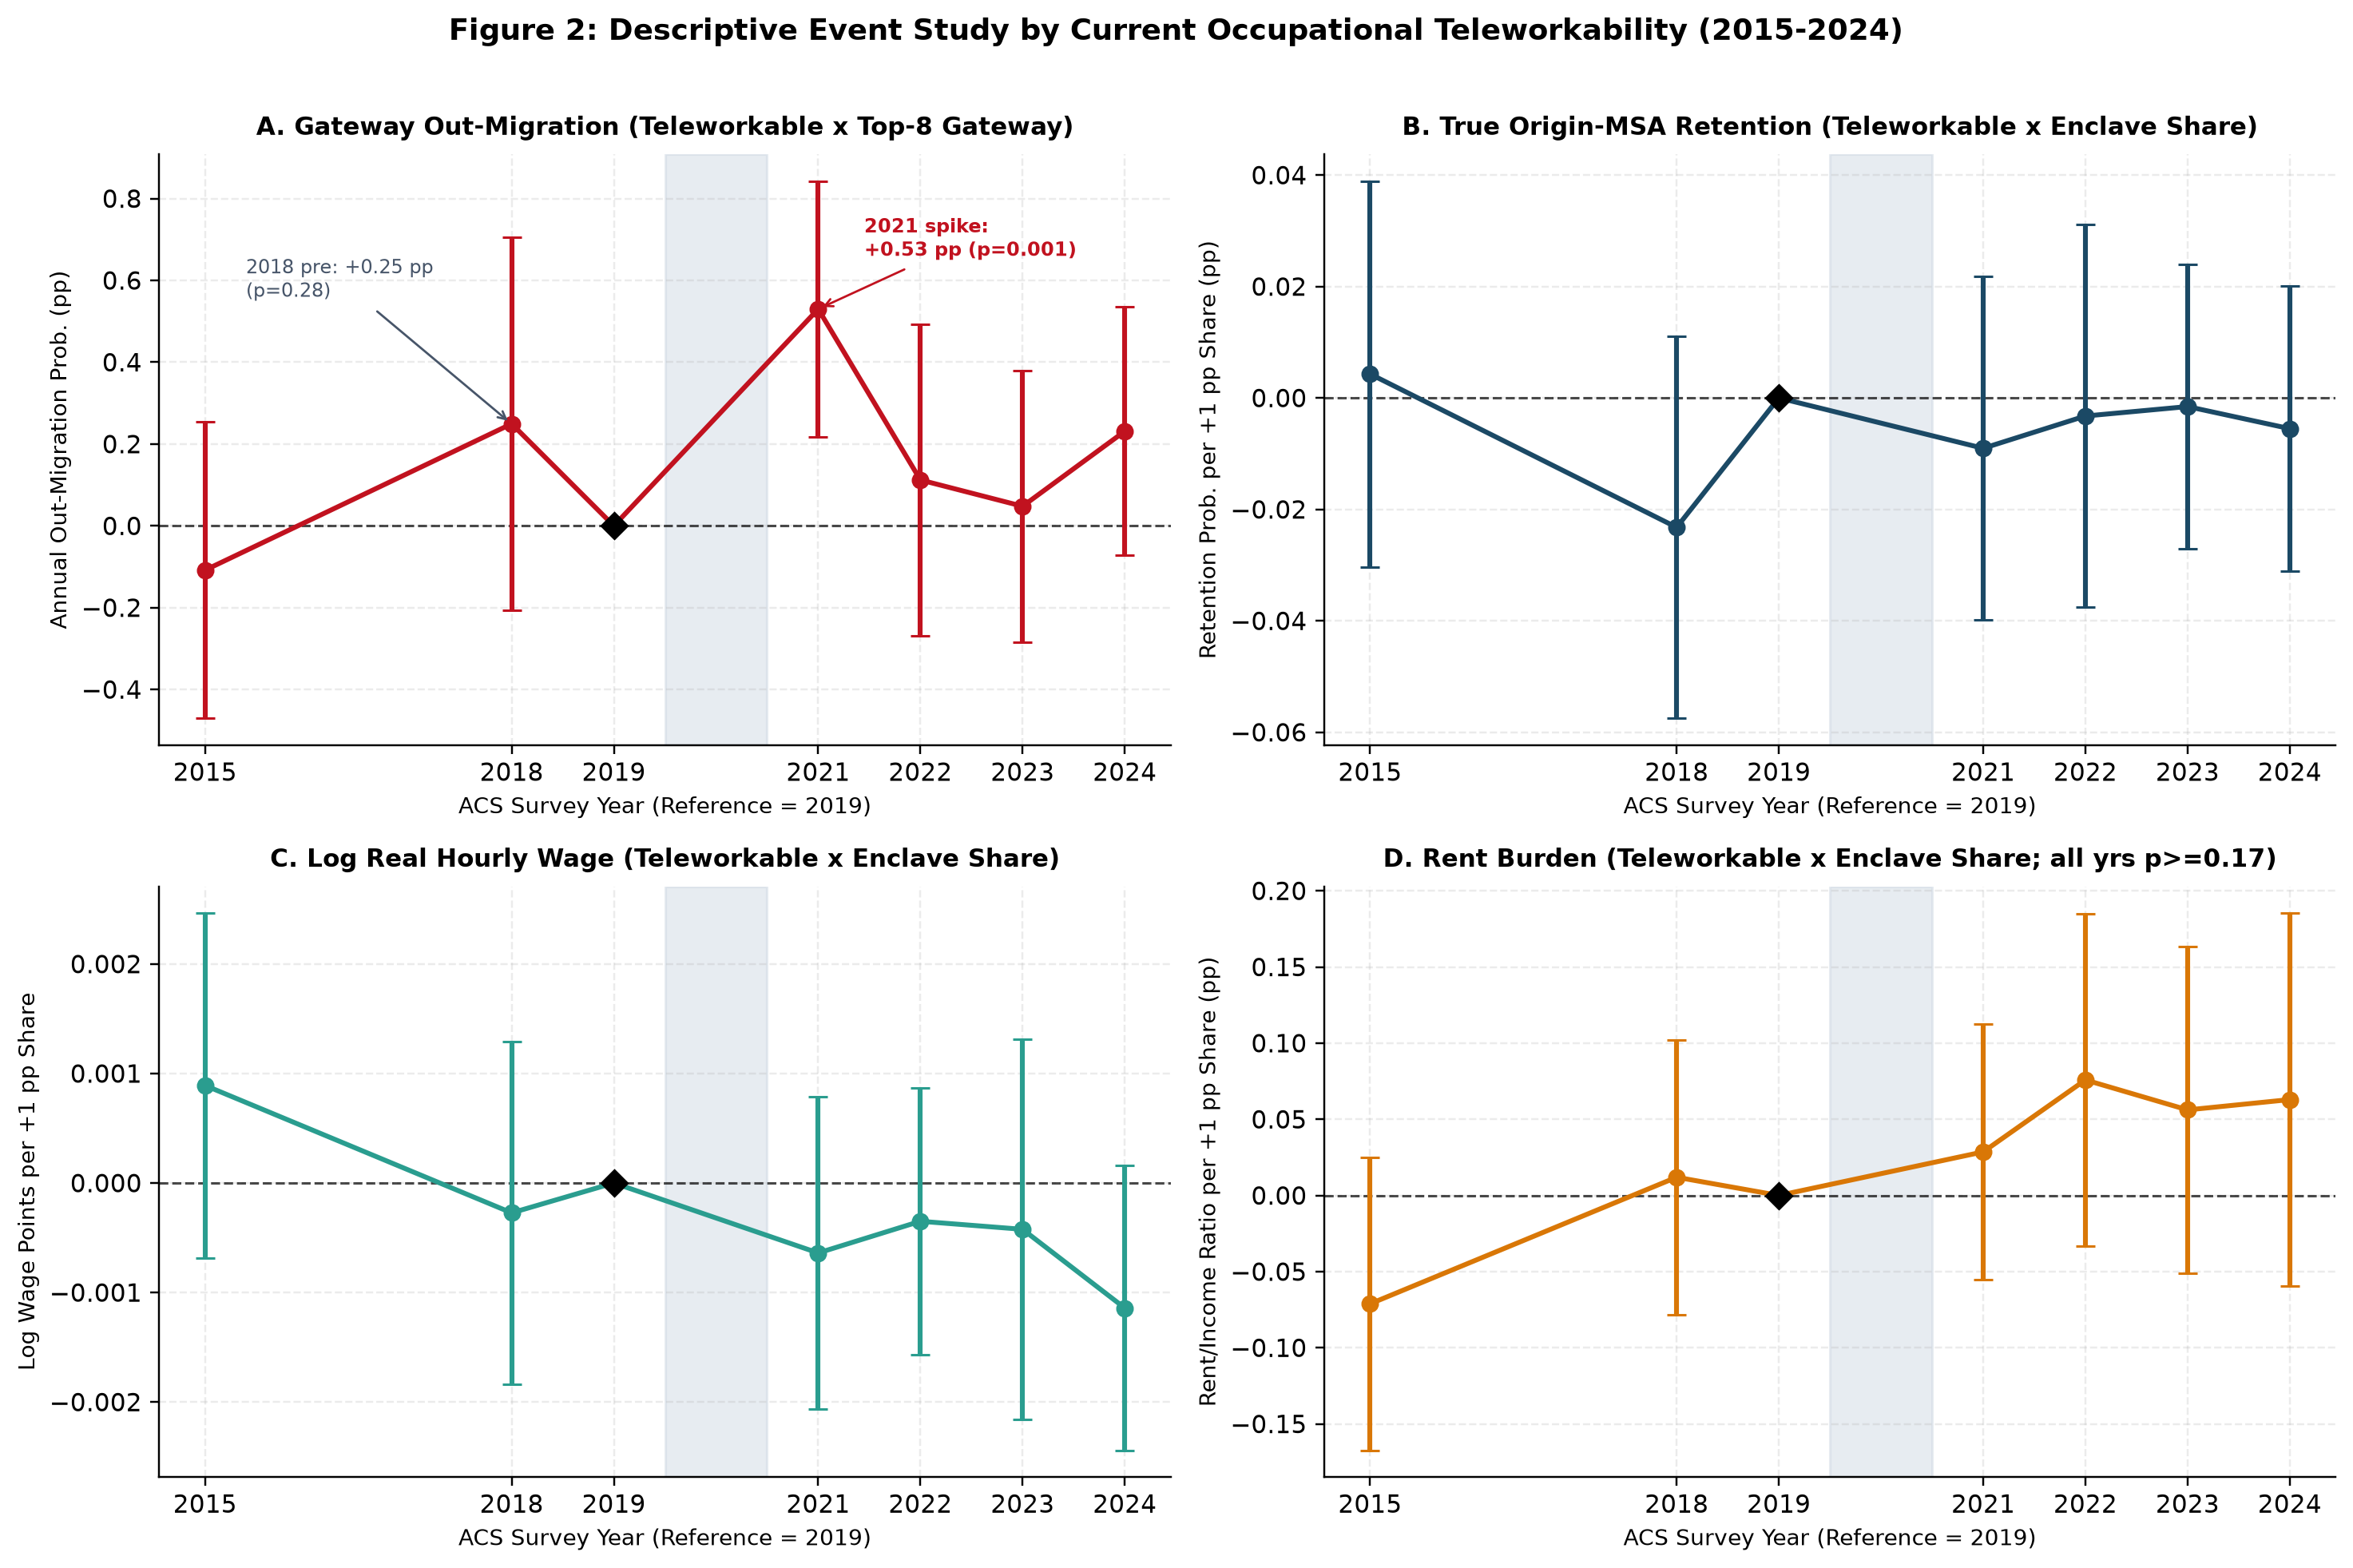
\includegraphics[width=0.90\linewidth,height=0.33\textheight,keepaspectratio]{figures/fig2_telework_event_study_2015_2024.png}
\caption{Descriptive Post-2020 Mobility, Retention, Wage, and Rent-Burden Event Studies, 2015--2024. \normalfont Reference year $= 2019$. Gateway out-migration by current occupational teleworkability displays a noisy 2018 pre-period point ($+0.25$ pp) and a single significant 2021 spike ($+0.53$ pp, $p = 0.001$) that reverted in 2022--2023. Origin-MSA retention sits near zero, and every annual rent-burden estimate is insignificant ($p \ge 0.17$).}
\label{fig:event_study}
\end{figure}

\section{Inter-MSA Mover Destinations: Testing Enclave Arbitrage and Sunbelt Relocation}

When co-ethnic natives left expensive gateways after 2020, did remote-capable or remote-working movers systematically relocate to affordable secondary Sunbelt enclaves such as Dallas--Fort Worth, Houston, Atlanta, Austin, Phoenix, Raleigh, or Charlotte? To test this, we analyze $99{,}329$ inter-MSA U.S.-born co-ethnic movers observed across 2015--2024 ($99{,}074$ in regression samples after fixed-effect singleton drops; $94{,}921$ with matched ZORI rent data), including $24{,}198$ exits from the top eight gateways ($24{,}129$ in regression samples) and $5{,}181$ exits from high-enclave gateways (origin co-ethnic share $\ge 1.0$ pp). Following our baseline typology, we define \emph{Enclave Arbitrage} as moving to a metro at least 10 percent cheaper in 2019 ZORI ($\Delta \ln \text{ZORI}_{2019} < -0.10$) with destination co-ethnic share $\ge 0.50$ pp, and \emph{Enclave Abandonment} as $\Delta \ln \text{ZORI}_{2019} < -0.10$ with destination share $< 0.50$ pp.

Crucially, gateway-exit regressions clustered by origin MSA have only $G = 8$ clusters, where standard asymptotic $t$-tests with seven degrees of freedom severely over-reject and statistical power is inherently limited. Table~\ref{tab:enclave_arbitrage} therefore reports restricted wild cluster bootstrap $p$-values using Webb (2023) 6-point weights ($9{,}999$ draws; Cameron, Gelbach, and Miller 2008) beside every asymptotic standard error.

\begin{table}[t!]
\centering
\caption{Inter-MSA Mover Destinations (\texttt{MIGMET131}, 2015--2024) with Webb 6-Point Wild Cluster Bootstrap $p$-Values}
\label{tab:enclave_arbitrage}
\scriptsize
\renewcommand{\arraystretch}{1.05}
\begin{tabular}{lccccccc}
\toprule
 & \multicolumn{3}{c}{$\text{Teleworkable} \times \text{Post}$} & \multicolumn{3}{c}{Realized $\text{WFH} \times \text{Post}$} & \\
\cmidrule(lr){2-4}\cmidrule(lr){5-7}
Destination Outcome ($\text{Dest} - \text{Orig}$) & Coef. & (SE) & [$p_{\text{WCB}}$] & Coef. & (SE) & [$p_{\text{WCB}}$] & $N$ \\
\midrule
\multicolumn{8}{l}{\textit{Panel A: All Inter-MSA Co-Ethnic Native Movers ($G = 259$--$266$ Origin MSAs)}} \\
$\Delta \ln(\text{ZORI Rent})$ & +0.0084 & (0.0053) & [0.128] & +0.0297*** & (0.0104) & [0.005] & 94,921 \\
$\Delta \ln(\text{Co-Ethnic Share})$ & -0.0106 & (0.0114) & [0.358] & +0.0362* & (0.0185) & [0.067] & 99,074 \\
$P(\text{Sunbelt Hub})$ & -0.0086 & (0.0077) & [0.273] & -0.0094 & (0.0137) & [0.503] & 99,074 \\
$P(\text{Enclave Arbitrage})$ & +0.0066 & (0.0040) & [0.102] & +0.0100 & (0.0072) & [0.172] & 99,074 \\
$P(\text{Enclave Abandonment})$ & -0.0093 & (0.0063) & [0.150] & -0.0202 & (0.0126) & [0.126] & 99,074 \\
\midrule
\multicolumn{8}{l}{\textit{Panel B: Movers Exiting Top-8 High-Cost Gateway MSAs ($G = 8$ Origin Clusters)}} \\
$\Delta \ln(\text{ZORI Rent})$ & -0.0047 & (0.0117) & [0.762] & +0.0230 & (0.0196) & [0.330] & 23,761 \\
$\Delta \text{Co-Ethnic Share}$ (pp) & -0.0257 & (0.1620) & [0.889] & +0.2224* & (0.0991) & [0.054] & 24,129 \\
$\Delta \ln(\text{Co-Ethnic Share})$ & -0.0230 & (0.0266) & [0.402] & +0.0716* & (0.0349) & [0.072] & 24,129 \\
$P(\text{Sunbelt Hub})$ & -0.0097 & (0.0165) & [0.574] & -0.0406 & (0.0263) & [0.174] & 24,129 \\
$P(\text{Enclave Arbitrage})$ & +0.0057 & (0.0075) & [0.430] & +0.0088 & (0.0105) & [0.405] & 24,129 \\
$P(\text{Enclave Abandonment})$ & -0.0117 & (0.0091) & [0.241] & -0.0333 & (0.0259) & [0.280] & 24,129 \\
\midrule
\multicolumn{8}{l}{\textit{Panel C: High-Enclave Gateway Exits (Origin Co-Ethnic Share $\ge 1.0$ pp; $G = 8$ Clusters)}} \\
$\Delta \text{Co-Ethnic Share}$ (pp) & +0.1719 & (0.5910) & [0.855] & +1.2517 & (0.7336) & [0.084] & 5,181 \\
$P(\text{Sunbelt Hub})$ & +0.0293 & (0.0276) & [0.301] & -0.0041 & (0.0572) & [0.944] & 5,181 \\
$P(\text{Enclave Arbitrage})$ & -0.0153 & (0.0335) & [0.725] & -0.0225 & (0.0406) & [0.620] & 5,181 \\
$P(\text{Enclave Abandonment})$ & +0.0123 & (0.0205) & [0.708] & -0.0494* & (0.0221) & [0.102] & 5,181 \\
\bottomrule
\end{tabular}
\begin{minipage}{0.98\linewidth}
\footnotesize\textit{Notes:} Inter-MSA native co-ethnic movers (\texttt{MIGMET131} $\ne$ \texttt{MET2013}, 2015--2024), controlling for Eth$\times$Yr and Origin-MSA FEs, age, education, and sex, weighted by \texttt{PERWT}. Standard errors clustered by Origin MSA; brackets report two-sided restricted wild cluster bootstrap $p$-values using Webb (2023) 6-point weights ($9{,}999$ draws; Cameron, Gelbach, and Miller 2008). Stars reflect asymptotic clustered $p$-values ($^{***}p<0.01$, $^{**}p<0.05$, $^{*}p<0.10$). Under Webb WCB, high-enclave gateway abandonment ($-0.0494$) rises to $p_{\text{WCB}} = 0.102$, and both Sunbelt and enclave-arbitrage estimates are negative or null.
\end{minipage}
\end{table}


Across Table~\ref{tab:enclave_arbitrage} and Figure~\ref{fig:arbitrage}, we find no consistent positive differential in Sunbelt relocation or high-enclave arbitrage among observed gateway leavers. The $26.5$--$38.8$ percent mean rent savings among gateway leavers are descriptive averages for \emph{all} gateway leavers rather than a remote-work premium: post-2020 non-teleworkable gateway leavers recorded larger mean rent reductions ($-30.9$ log points) than teleworkable leavers ($-26.5$ log points), and across all movers realized remote workers relocated to slightly \emph{higher}-rent destinations ($+0.0297^{***}$, $p_{\text{WCB}} = 0.005$).

Among gateway leavers (Panel B), the direct Sunbelt relocation probability carries negative and imprecisely estimated point estimates under both occupational teleworkability ($-0.0097$, $p_{\text{WCB}} = 0.574$) and realized work-from-home ($-0.0406$, $p_{\text{WCB}} = 0.174$). Among high-enclave gateway exits (Panel C), the enclave-arbitrage estimate is likewise negative and indistinguishable from zero under both teleworkability ($-0.0153$, $p_{\text{WCB}} = 0.725$) and realized work-from-home ($-0.0225$, $p_{\text{WCB}} = 0.620$), though wide confidence bands with eight origin clusters prevent ruling out modest effects. Realized work-from-home gateway leavers do show marginally higher destination co-ethnic density ($+0.222$ pp, $p_{\text{WCB}} = 0.054$; $+0.0716$ in logs, $p_{\text{WCB}} = 0.072$) relative to on-site leavers, but those endogenous work-from-home estimates do not appear under occupational teleworkability ($-0.0230$, $p_{\text{WCB}} = 0.402$), and the high-enclave realized-WFH abandonment reduction ($-0.0494$, asymptotic $p = 0.060$) loses 10 percent significance under Webb wild cluster bootstrap inference ($p_{\text{WCB}} = 0.102$).

\begin{figure}[t!]
\centering
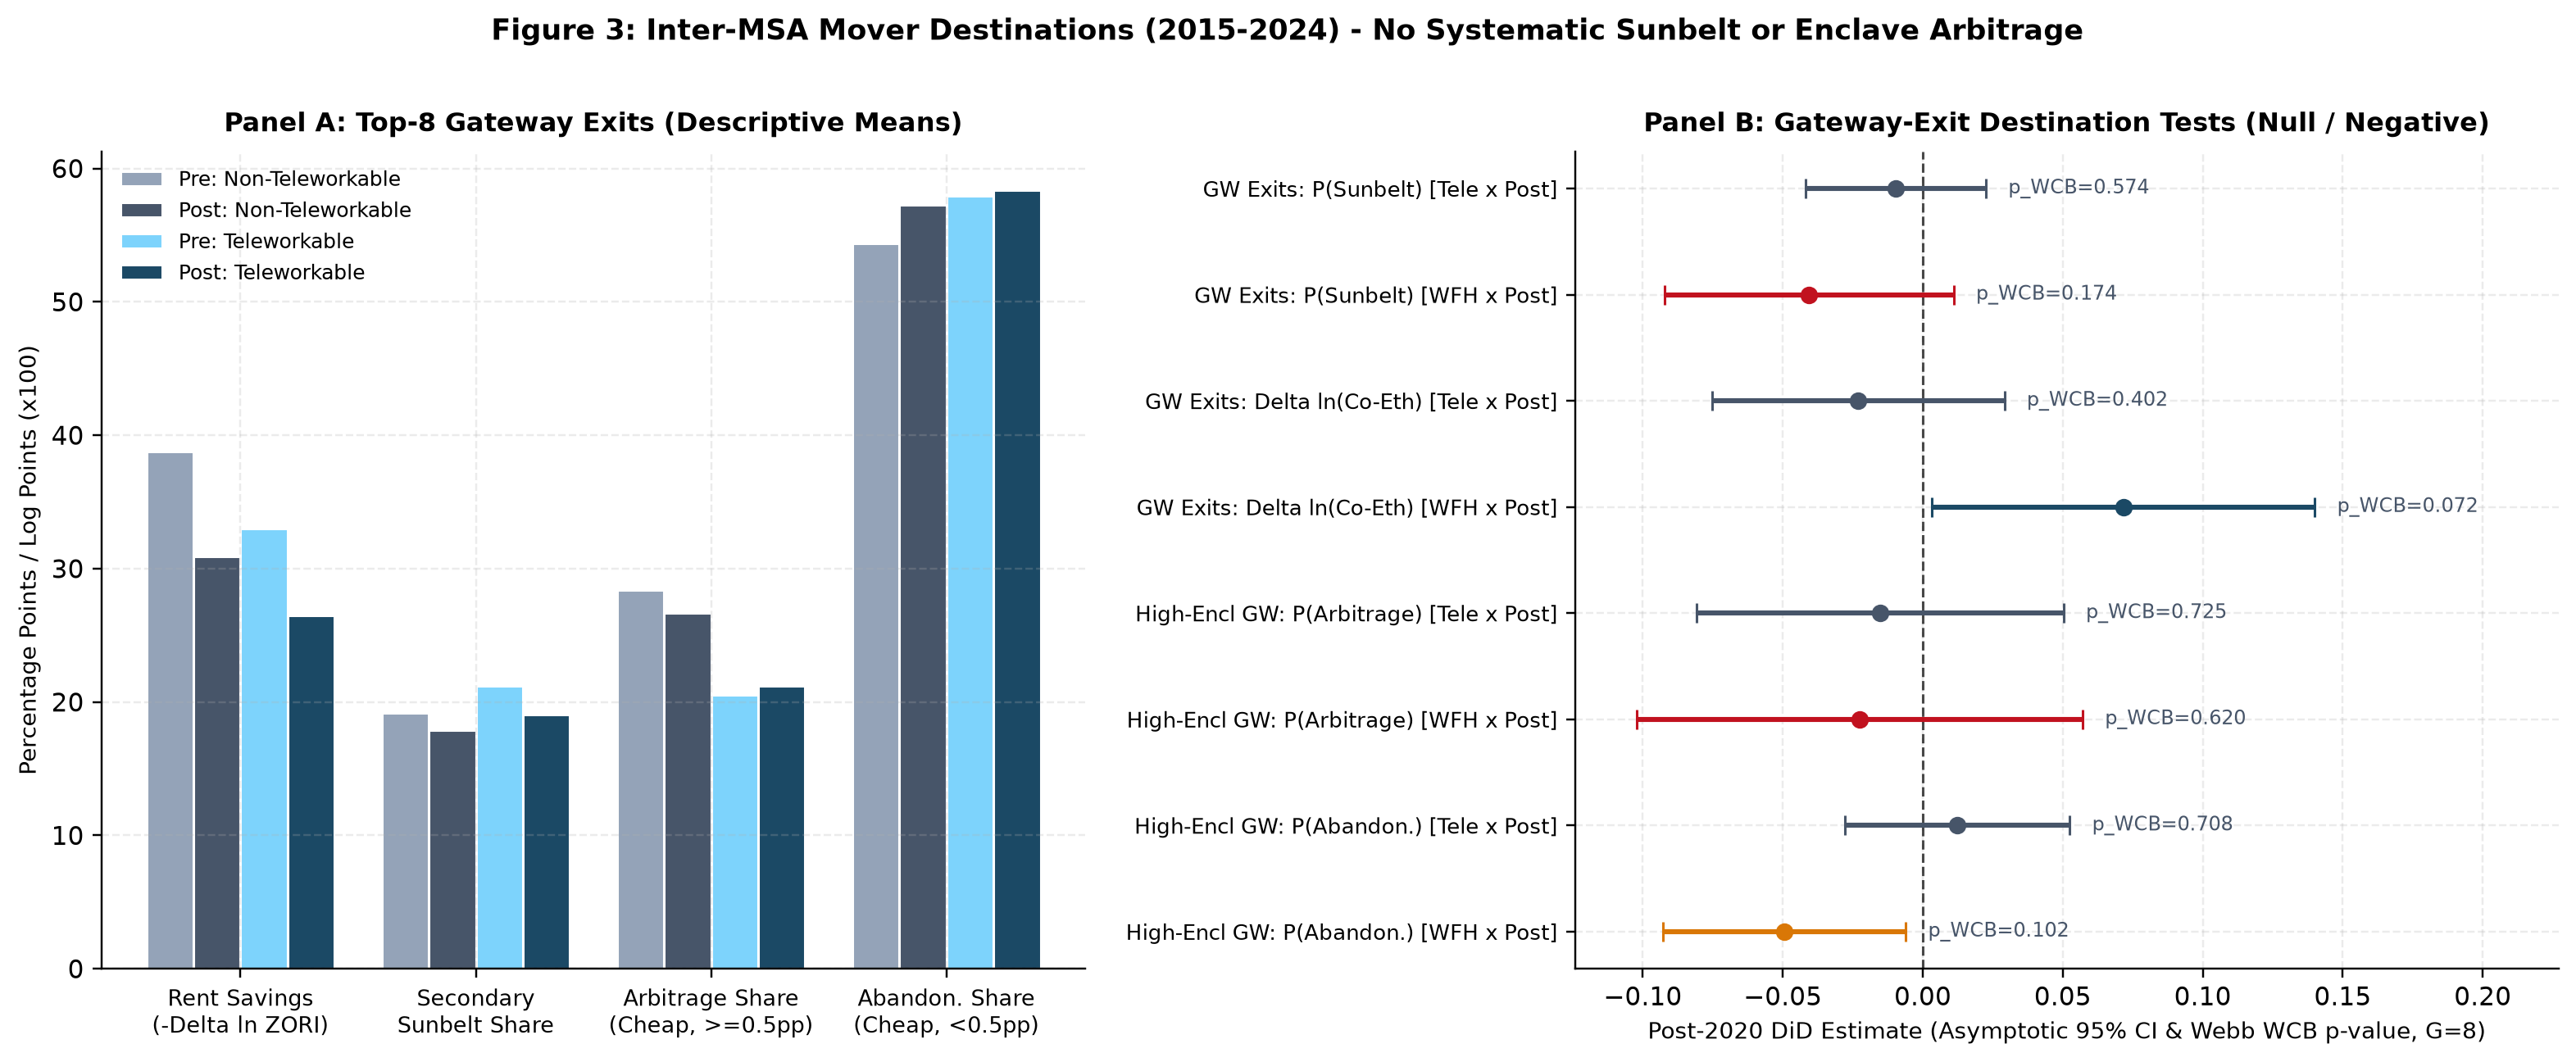
\includegraphics[width=0.90\linewidth,height=0.33\textheight,keepaspectratio]{figures/fig3_enclave_arbitrage_vs_abandonment.png}
\caption{Inter-MSA Mover Destinations, Sunbelt Relocation, and Enclave Arbitrage, 2015--2024. \normalfont Panel~A displays descriptive gateway-exit means (showing large rent drops for all leavers). Panel~B plots difference-in-differences estimates with asymptotic 95 percent CIs and Webb 6-point wild cluster bootstrap $p$-values ($G = 8$): Sunbelt relocation and high-enclave arbitrage estimates are negative with wide uncertainty, and realized-WFH abandonment reaches $p_{\text{WCB}} = 0.102$.}
\label{fig:arbitrage}
\end{figure}

To verify that these null results do not depend on arbitrary cutoffs, Table~\ref{tab:sensitivity_grid} reports a pre-specified sensitivity grid for high-enclave gateway exits across nine one-way specification checks (seven distinct configurations around the baseline), varying the gateway set (Top 5, Top 8, Top 12), the rent-savings threshold (5, 10, and 15 percent), and the destination co-ethnic share threshold (0.25, 0.50, and 1.00 pp). Across every configuration, not a single enclave-arbitrage estimate is positive and statistically significant under Webb WCB (the lone estimate clearing $p_{\text{WCB}} < 0.10$ is negative, at $-0.0626$, $p_{\text{WCB}} = 0.09$ under the 0.25 pp co-ethnic cutoff for realized WFH). Enclave abandonment is similarly null across all teleworkable specifications ($p_{\text{WCB}} \ge 0.19$) and in all but the Top-12 realized-WFH specification ($p_{\text{WCB}} = 0.056$).

\begin{table}[t!]
\centering
\caption{Pre-Specified Sensitivity Grid for High-Enclave Gateway Exits (Coefficients and Webb WCB $p$-Values)}
\label{tab:sensitivity_grid}
\footnotesize
\renewcommand{\arraystretch}{1.05}
\begin{tabular}{lcccc}
\toprule
 & \multicolumn{2}{c}{$P(\text{Enclave Arbitrage})$} & \multicolumn{2}{c}{$P(\text{Enclave Abandonment})$} \\
\cmidrule(lr){2-3}\cmidrule(lr){4-5}
Sensitivity Specification & Tele $\times$ Post & WFH $\times$ Post & Tele $\times$ Post & WFH $\times$ Post \\
\midrule
Gateways: Top 5 ($G=5$) & -0.0185 [0.69] & -0.0144 [0.72] & +0.0150 [0.69] & -0.0420 [0.20] \\
Gateways: Top 8 (Baseline, $G=8$) & -0.0153 [0.72] & -0.0225 [0.62] & +0.0123 [0.71] & -0.0494 [0.10] \\
Gateways: Top 12 ($G=12$) & -0.0124 [0.69] & -0.0256 [0.54] & +0.0046 [0.87] & -0.0535 [0.06] \\
\midrule
Rent Cutoff: $\ge 5\%$ Cheaper & +0.0047 [0.91] & -0.0189 [0.69] & +0.0131 [0.67] & -0.0331 [0.33] \\
Rent Cutoff: $\ge 10\%$ (Baseline) & -0.0153 [0.72] & -0.0225 [0.62] & +0.0123 [0.71] & -0.0494 [0.10] \\
Rent Cutoff: $\ge 15\%$ Cheaper & -0.0179 [0.55] & +0.0118 [0.81] & +0.0079 [0.79] & -0.0371 [0.20] \\
\midrule
Co-Ethnic Cutoff: $\ge 0.25$ pp & -0.0206 [0.40] & -0.0626 [0.09] & +0.0176 [0.19] & -0.0094 [0.50] \\
Co-Ethnic Cutoff: $\ge 0.50$ pp (Base) & -0.0153 [0.72] & -0.0225 [0.62] & +0.0123 [0.71] & -0.0494 [0.10] \\
Co-Ethnic Cutoff: $\ge 1.00$ pp & +0.0068 [0.83] & -0.0307 [0.33] & -0.0099 [0.67] & -0.0413 [0.14] \\
\bottomrule
\end{tabular}
\begin{minipage}{0.96\linewidth}
\footnotesize\textit{Notes:} Each cell reports the DiD coefficient followed by its Webb 6-point wild cluster bootstrap $p$-value ($9{,}999$ draws) in brackets for high-enclave gateway exits (origin co-ethnic share $\ge 1.0$ pp). Top 5: NYC, LA, SF, Chicago, Miami. Top 8 adds DC, Boston, Seattle. Top 12 adds Houston, Dallas--Fort Worth, San Diego, San Jose. Across all nine configurations, no arbitrage estimate is positive and significant, and only Top-12 WFH abandonment reaches $p_{\text{WCB}} = 0.056$.
\end{minipage}
\end{table}


\section{Weak-IV Audit of Shift-Share Identification (1980--2024)}

We conclude our empirical analysis with a weak-IV audit of the shift-share identification strategy in Song and Xu (2020) and Song (2017), drawing on the shift-share and weak-instrument literature (Card and Peri 2016; Jaeger, Ruist, and Stuhler 2018; Ad\~{a}o, Koles\'{a}r, and Morales 2019; Goldsmith-Pinkham, Sorkin, and Swift 2020; Borusyak, Hull, and Jaravel 2022). Pooling 1980--2010 Decennial waves with 2019 and 2024 ACS waves mixes 10-year lags with 9-year and 5-year lags and combines 5-year Census migration windows with 1-year ACS migration windows, rendering lag structures non-comparable across waves. We therefore separate two panels in Table~\ref{tab:jrs_weak_iv} and Figure~\ref{fig:weak_iv}: Panel A uses a uniform 10-year decadal panel (1980, 1990, 2000, and 2010, with exact 10-year lags in 2000 and 2010 and 5-year retention restricted strictly to 1980--2000 Census waves), while Panel B reports the modern ACS extension (2010, 2019, and 2024, uniform 1-year migration window) separately.

Every model absorbs ethnicity-by-year, metro-by-year, and ethnicity-by-metro fixed effects via weighted Frisch--Waugh--Lovell projections, with two-way (MSA $\times$ ethnicity) clustered standard errors (Cameron, Gelbach, and Miller 2011) and Sanderson and Windmeijer (2016) conditional $F$-statistics. For every single-endogenous-variable (1-IV) specification, we invert the exact cluster-robust Anderson and Rubin (1949) / Finlay and Magnusson (2009) statistic analytically in closed form via the quadratic inequality:
\begin{equation}
(s_d^2 - c v_{dd})\beta^2 - 2(s_y s_d - c v_{yd})\beta + (s_y^2 - c v_{yy}) \le 0, \qquad c = \chi^2_{1,0.95},
\end{equation}
avoiding artificial finite grid clipping. Whenever SW $F < 3.84$, the leading quadratic coefficient is negative and the exact 95 percent Anderson--Rubin (AR) confidence set is strictly unbounded: either a disconnected union $(-\infty, r_1] \cup [r_2, +\infty)$ or the entire real line $(-\infty, +\infty)$. All two-instrument projected AR sets in Panel A are verified strictly interior to their two-dimensional search grids.

\begin{table}[t!]
\centering
\caption{Weak-IV-Robust Shift-Share Inference: Uniform 10-Year Decadal Panel vs.\ Separate ACS Extension}
\label{tab:jrs_weak_iv}
\scriptsize
\setlength{\tabcolsep}{3.1pt}
\renewcommand{\arraystretch}{1.05}
\begin{tabular}{lllccccc}
\toprule
Outcome & Model & Inflow & Coef. & (2-Way SE) & SW $F$ & Exact AR 95\% Set & $N$ \\
\midrule
\multicolumn{8}{l}{\textit{Panel A: Uniform 10-Year Decadal Panel (1980, 1990, 2000, 2010; Exact 10-Yr Lags; 5-Yr Retention 1980--2000)}} \\
$\ln(\text{Residents})$ & Static 1-IV & Contemp. & +0.0176* & (0.0094) & 120.2 & $[-0.002,\,+0.036]$ & 13,457 \\
$\ln(\text{Residents})$ & JRS 2-IV & Contemp. & +0.0351 & (0.0252) & 25.0 & $[-0.050,\,+0.097]$ & 9,010 \\
$\ln(\text{Residents})$ & JRS 2-IV & Lagged & -0.0047 & (0.0422) & 19.0 & $[-0.148,\,+0.091]$ & 9,010 \\
$\ln(\text{OOS Residents})$ & Static 1-IV & Contemp. & +0.0321*** & (0.0096) & 113.3 & $[+0.013,\,+0.051]$ & 12,182 \\
$\ln(\text{OOS Residents})$ & JRS 2-IV & Contemp. & +0.0553* & (0.0313) & 28.2 & $[-0.051,\,+0.126]$ & 8,141 \\
$\ln(\text{OOS Residents})$ & JRS 2-IV & Lagged & +0.0020 & (0.0512) & 21.8 & $[-0.172,\,+0.108]$ & 8,141 \\
$\ln(\text{Hourly Wage})$ & Static 1-IV & Contemp. & +0.2518 & (1.3165) & 0.0 & $(-\infty, -0.018] \cup [+0.022, +\infty)$ & 13,784 \\
$\ln(\text{Hourly Wage})$ & JRS 2-IV & Contemp. & -0.0116*** & (0.0037) & 11.4 & $[-0.040,\,+0.007]$ & 9,168 \\
$\ln(\text{Hourly Wage})$ & JRS 2-IV & Lagged & +0.0100 & (0.0072) & 13.8 & $[-0.005,\,+0.036]$ & 9,168 \\
True Retention (5-Yr) & Static 1-IV & Contemp. & -0.0472 & (0.0742) & 0.7 & $(-\infty, +\infty)$ & 9,667 \\
\midrule
\multicolumn{8}{l}{\textit{Panel B: Modern ACS Extension Panel (2010, 2019, 2024; Uniform 1-Year ACS Migration Window)}} \\
$\ln(\text{Residents})$ & Static 1-IV & Contemp. & +0.0158** & (0.0071) & 320.8 & $[+0.003,\,+0.031]$ & 13,580 \\
$\ln(\text{OOS Residents})$ & Static 1-IV & Contemp. & +0.0252*** & (0.0076) & 264.5 & $[+0.011,\,+0.041]$ & 12,094 \\
True Retention (1-Yr) & Static 1-IV & Contemp. & -0.0031 & (0.0036) & 0.7 & $(-\infty, +0.0000] \cup [+0.0004, +\infty)$ & 13,740 \\
$\ln(\text{Hourly Wage})$ & Static 1-IV & Contemp. & -0.0114 & (0.0209) & 0.8 & $(-\infty, +\infty)$ & 13,342 \\
\bottomrule
\end{tabular}
\begin{minipage}{0.98\linewidth}
\footnotesize\textit{Notes:} Balanced (\texttt{eth}, \texttt{met2013}, \texttt{year}) panels with Eth$\times$Yr, MSA$\times$Yr, and Eth$\times$MSA FEs absorbed via weighted FWL projections. Panel A uses exact 10-year decadal spacing (Static 1-IV on 1990--2010; JRS 2-IV on 2000--2010) and restricts 5-year retention strictly to 1980--2000 Census waves. Panel B reports the 2010--2019--2024 ACS extension separately (uniform 1-year migration window, Static 1-IV on 2019--2024). Two-way clustered SEs (MSA $\times$ Ethnicity) and Sanderson--Windmeijer (2016) conditional $F$-statistics. All 1-IV Anderson--Rubin (1949) 95\% confidence sets are solved analytically in closed form without finite grid clipping, yielding unbounded unions or $(-\infty, +\infty)$ whenever SW $F < 3.84$; all 2-IV projected sets are verified strictly interior to their 2D search grids. $^{***}p<0.01$, $^{**}p<0.05$, $^{*}p<0.10$.
\end{minipage}
\end{table}


This exact audit draws a sharp boundary between well-identified and weakly identified estimands. Out-of-state-born adult clustering ($\ln(\text{OOS Residents})$, which excludes locally born children growing up in place) is strongly positive and tightly bounded under static 1-IV leave-out Bartik in both the uniform 1980--2010 decadal panel ($+0.0321^{***}$, SW $F = 113.3$, exact AR 95 percent set $[+0.013, +0.051]$) and the 2010--2024 ACS extension ($+0.0252^{***}$, SW $F = 264.5$, exact AR 95 percent set $[+0.011, +0.041]$). Total $\ln(\text{Residents})$ is likewise bounded in both panels, with a strictly positive 95 percent AR set in the ACS ($+0.0158^{**}$, $[+0.003, +0.031]$) and a bounded set marginally spanning zero in the decadal panel ($+0.0176^{*}$, $[-0.002, +0.036]$); PPML checks (Santos Silva and Tenreyro 2006) confirm that retaining zero-resident cells preserves the positive sign.

In the uniform 10-year dynamic JRS two-instrument specification (2000 and 2010), point estimates continue to show a positive contemporaneous pull for out-of-state-born adults ($+0.0553^{*}$, SW $F = 28.2$) alongside a near-zero lagged inflow coefficient ($+0.0020$, SW $F = 21.8$). With only two uniform decadal estimation waves, however, the bounded 2D-projected Anderson--Rubin 95 percent confidence interval widens to $[-0.051, +0.126]$ (Figure~\ref{fig:weak_iv} Panel B shows the diagonal correlation ridge, although the joint 2D region still excludes $(0,0)$).

By contrast, population-weighted retention and static wage IVs lose first-stage power once uneven lags and migration windows are separated. Pure 5-year Census retention (1980--2000, SW $F = 0.7$) and modern ACS static wages (2010--2024, SW $F = 0.8$) yield the entire real line $(-\infty, +\infty)$ as their exact 95 percent AR confidence set. Decadal static wages (SW $F = 0.0$) yield the unbounded disconnected union $(-\infty, -0.018] \cup [+0.022, +\infty)$, and 1-year ACS retention (SW $F = 0.7$) yields $(-\infty, +0.0000] \cup [+0.0004, +\infty)$. Even in the decadal dynamic JRS wage specification, where the Wald test appears significant ($-0.0116^{***}$, SE $0.0037$) at SW $F = 11.4$, the exact bounded 2D-projected AR 95 percent interval is $[-0.040, +0.007]$ and spans zero. Reporting exact analytical AR sets thus clarifies where shift-share IV genuinely identifies co-ethnic clustering versus where instruments are uninformative.

\begin{figure}[t!]
\centering
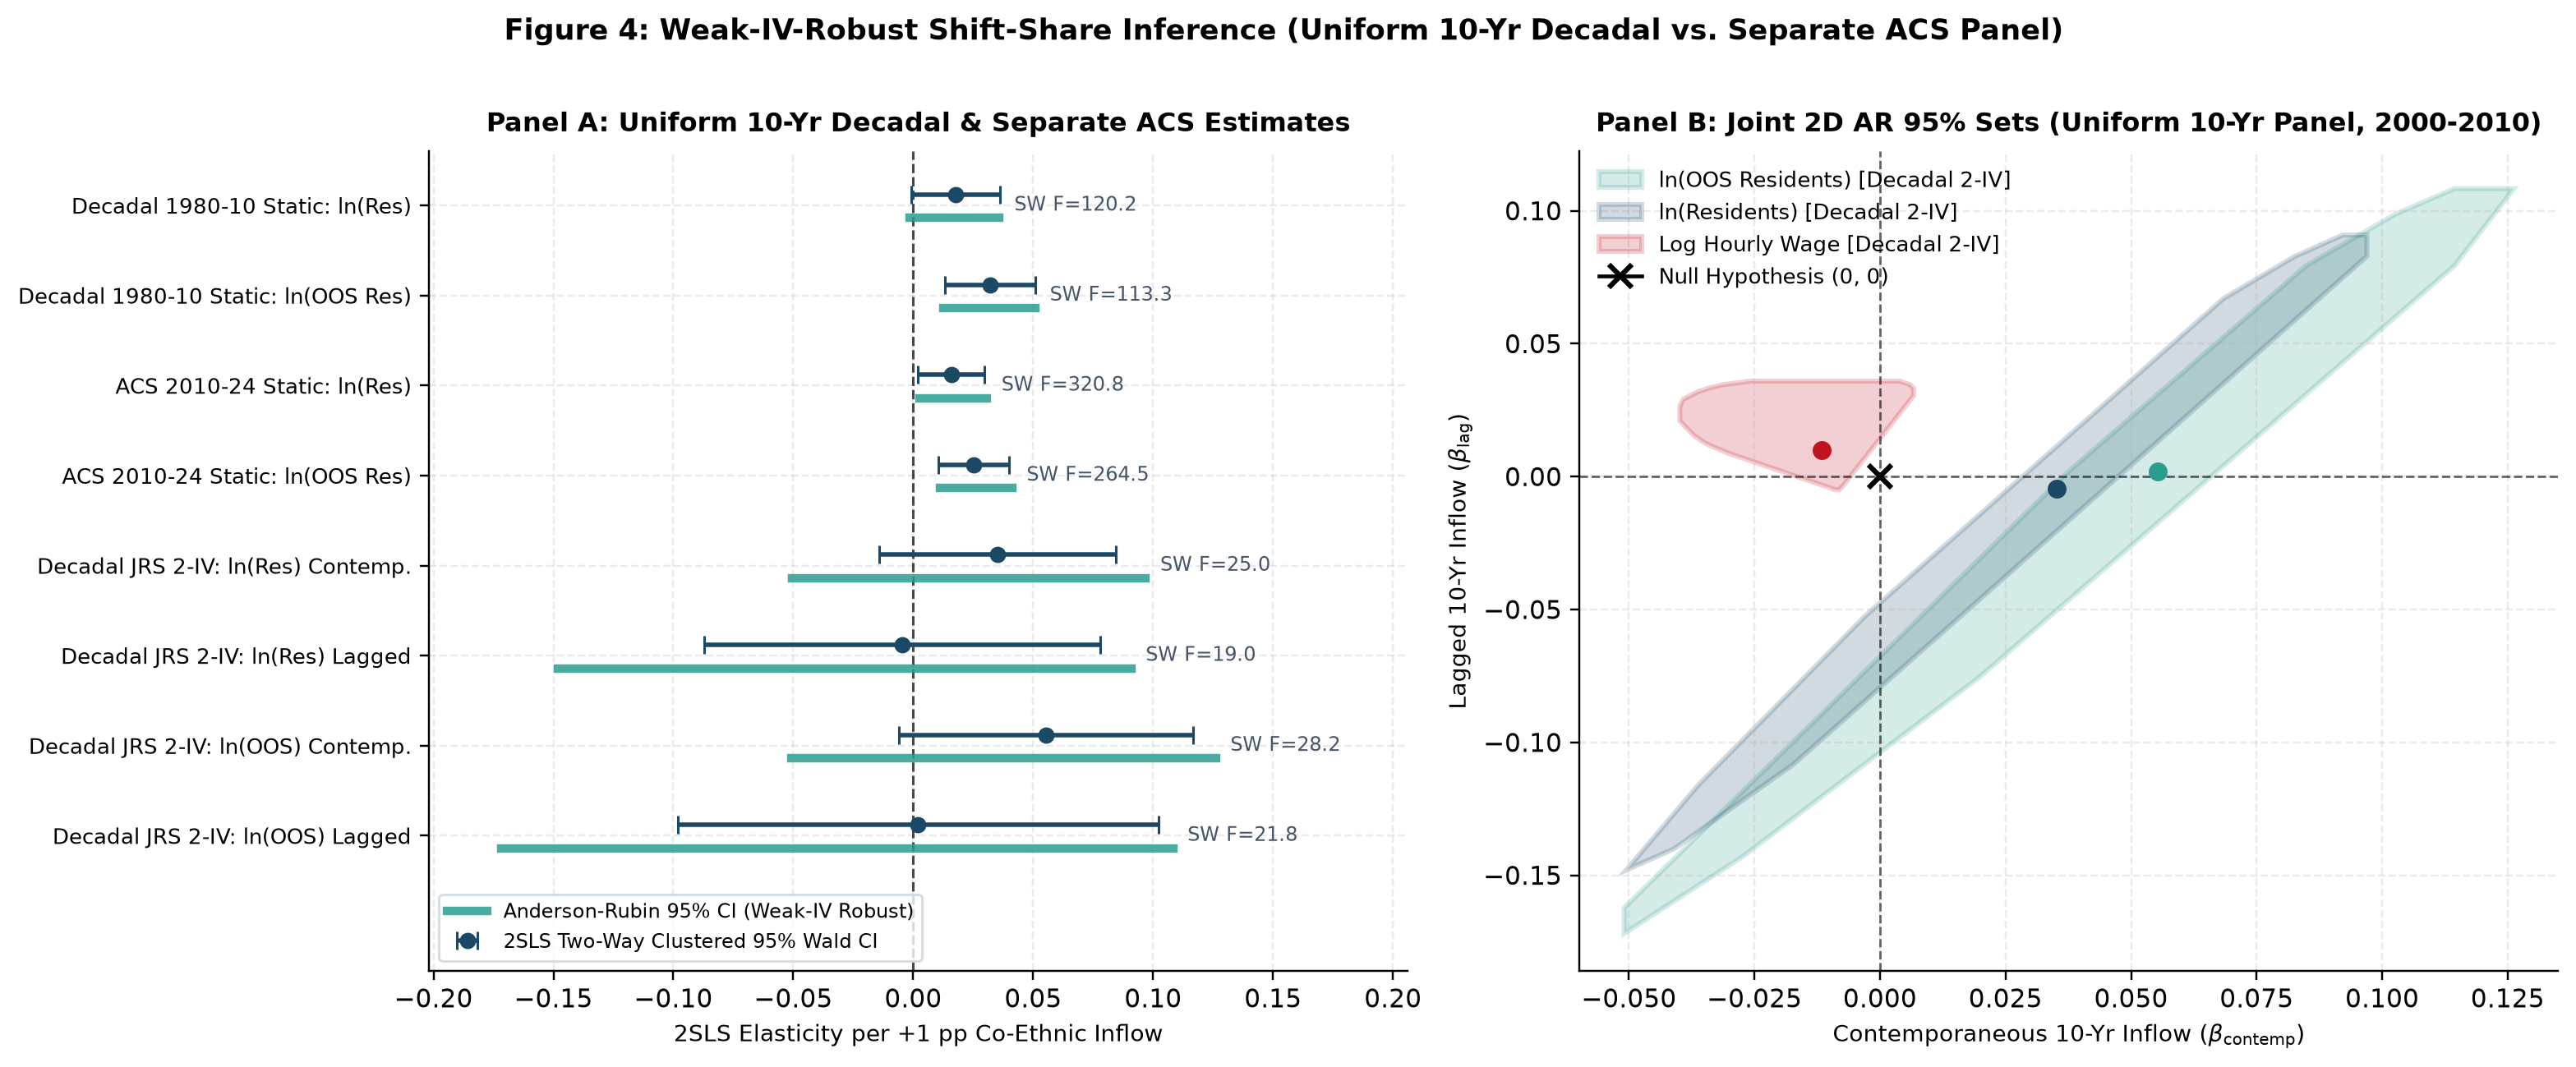
\includegraphics[width=0.90\linewidth,height=0.33\textheight,keepaspectratio]{figures/fig4_jrs_weak_iv_robust.png}
\caption{Weak-IV-Robust Shift-Share Inference Across Uniform Decadal and ACS Panels. \normalfont Panel~A compares two-way clustered Wald and exact bounded Anderson--Rubin 95 percent confidence intervals with Sanderson--Windmeijer conditional $F$-statistics for resident stock outcomes. Panel~B plots exact bounded 2D joint AR 95 percent regions on the uniform 10-year decadal panel (2000--2010).}
\label{fig:weak_iv}
\end{figure}

\FloatBarrier
\section{Conclusion}

Re-examining ethnic enclave persistence from 1980 through 2024 alongside Song and Xu (2020) and Song (2017) separates durable empirical regularities from fragile claims. Within metropolitan areas, consistent sub-metro regressions on unique households show no detectable rent or home-value discount with immigrant share even when endogenous room counts are excluded, while household crowding and three-or-more-generation households rise clearly and U.S.-born co-ethnic working-age adults experience higher crowding ($t = 2.20$). Common-sample dynamic-panel checks confirm severe downward Nickell (1981) bias in lagged-level price regressions ($\hat{\rho}_{\text{FE}} = -0.31$ versus $\hat{\rho}_{\text{AH}} = -0.003$ for rent; $-0.25$ versus $+0.063$ for home value), while recognizing that coarser PUMA-level OLS cannot rule out the tract-level neighborhood appreciation gaps documented by Saiz and Wachter (2011).

Turning to the post-2020 remote-work era, the data do not support causal claims of sustained remote-work gateway flight or systematic enclave arbitrage into Sunbelt hubs. Descriptive gateway-exit estimates by current occupational teleworkability rest on a single transitory 2021 spike ($+0.53$ pp) beside a noisy 2018 pre-period point ($+0.25$ pp), whereas pre-2019 origin-metro telework exposure predicts broader out-migration without any differential gateway effect. Across inter-metro movers, Webb 6-point wild cluster bootstrap inference ($G = 8$) and a pre-specified sensitivity grid find no consistent positive differential in Sunbelt relocation or enclave arbitrage among observed gateway leavers. Finally, exact analytical Anderson--Rubin inference on separated uniform decadal (1980--2010) and modern ACS (2010--2024) shift-share panels confirms tightly bounded positive out-of-state-born adult clustering under static Bartik IV in both eras, while showing that retention and static wage IVs yield unbounded confidence sets.

\section*{Acknowledgments}
This research was directed by Daksh Tyagi and carried out by a swarm of Gemini 4 Neon agents. Daksh Tyagi conceived the research agenda, supervised the econometric audits, and bears responsibility for the final manuscript.

\section*{References}
\small
\begin{list}{}{%
  \setlength{\leftmargin}{1.5em}%
  \setlength{\itemindent}{-1.5em}%
  \setlength{\itemsep}{0.14em}%
  \setlength{\parsep}{0pt}%
}
\item Ad\~{a}o, Rodrigo, Michal Koles\'{a}r, and Eduardo Morales. 2019. ``Shift-Share Designs: Theory and Inference.'' \emph{Quarterly Journal of Economics} 134(4): 1949--2010.
\item Anderson, Theodore W., and Cheng Hsiao. 1981. ``Estimation of Dynamic Models with Error Components.'' \emph{Journal of the American Statistical Association} 76(375): 598--606.
\item Anderson, Theodore W., and Herman Rubin. 1949. ``Estimation of the Parameters of a Single Equation in a Complete System of Stochastic Equations.'' \emph{Annals of Mathematical Statistics} 20(1): 46--63.
\item Barrero, Jose Maria, Nicholas Bloom, and Steven J.\ Davis. 2021. ``Why Working from Home Will Stick.'' NBER Working Paper No.\ 28731.
\item Borjas, George J. 2003. ``The Labor Demand Curve Is Downward Sloping: Reexamining the Impact of Immigration on the Labor Market.'' \emph{Quarterly Journal of Economics} 118(4): 1335--1374.
\item Borjas, George J. 2006. ``Native Internal Migration and the Labor Market Impact of Immigration.'' \emph{Journal of Human Resources} 41(2): 221--258.
\item Borusyak, Kirill, Peter Hull, and Xavier Jaravel. 2022. ``Quasi-Experimental Shift-Share Research Designs.'' \emph{Review of Economic Studies} 89(1): 181--213.
\item Cameron, A.\ Colin, Jonah B.\ Gelbach, and Douglas L.\ Miller. 2008. ``Bootstrap-Based Improvements for Inference with Clustered Errors.'' \emph{Review of Economics and Statistics} 90(3): 414--427.
\item Cameron, A.\ Colin, Jonah B.\ Gelbach, and Douglas L.\ Miller. 2011. ``Robust Inference with Multiway Clustering.'' \emph{Journal of Business \& Economic Statistics} 29(2): 238--249.
\item Card, David. 2001. ``Immigrant Inflows, Native Outflows, and the Local Labor Market Impacts of Higher Immigration.'' \emph{Journal of Labor Economics} 19(1): 22--64.
\item Card, David. 2009. ``Immigration and Inequality.'' \emph{American Economic Review} 99(2): 1--21.
\item Card, David, and Giovanni Peri. 2016. ``Immigration Economics by George J.\ Borjas: A Review Essay.'' \emph{Journal of Economic Literature} 54(4): 1333--1349.
\item Dingel, Jonathan I., and Brent Neiman. 2020. ``How Many Jobs Can Be Done at Home?'' \emph{Journal of Public Economics} 189: 104235.
\item Duncan, Brian, and Stephen J.\ Trejo. 2011a. ``Intermarriage and the Intergenerational Transmission of Ethnic Identity and Human Capital for Mexican Americans.'' \emph{Journal of Labor Economics} 29(2): 195--227.
\item Duncan, Brian, and Stephen J.\ Trejo. 2011b. ``Who Remains Mexican? Selective Ethnic Attrition and the Intergenerational Progress of Mexican Americans.'' In \emph{Latinos and the Economy}, ed.\ David L.\ Leal and Stephen J.\ Trejo, 285--320. New York: Springer.
\item Duncan, Brian, and Stephen J.\ Trejo. 2017. ``The Complexity of Immigrant Generations: Implications for Assessing the Socioeconomic Integration of Hispanics and Asians.'' \emph{ILR Review} 70(5): 1146--1175.
\item Federal Housing Finance Agency (FHFA). 2026. \emph{All-Transactions House Price Index (Metropolitan Statistical Areas, 1975--2026)}. Washington, DC: FHFA.
\item Finlay, Keith, and Leandro M.\ Magnusson. 2009. ``Implementing Weak Instrument Robust Tests for a General Class of Instrumental-Variables Models.'' \emph{Stata Journal} 9(3): 398--421.
\item Goldsmith-Pinkham, Paul, Isaac Sorkin, and Henry Swift. 2020. ``Bartik Instruments: What, When, Why, and How.'' \emph{American Economic Review} 110(8): 2586--2624.
\item Jaeger, David A., Joakim Ruist, and Jan Stuhler. 2018. ``Shift-Share Instruments and the Impact of Immigration.'' NBER Working Paper No.\ 24285.
\item National Center for O*NET Development. 2026. \emph{O*NET 31.0 Database: Generalized Work Activities}. U.S.\ Department of Labor.
\item Nickell, Stephen. 1981. ``Biases in Dynamic Models with Fixed Effects.'' \emph{Econometrica} 49(6): 1417--1426.
\item Peri, Giovanni, and Chad Sparber. 2011. ``Assessing Inherent Model Bias: An Application to Native Displacement in Response to Immigration.'' \emph{Journal of Urban Economics} 69(1): 82--91.
\item Ramani, Arjun, and Nicholas Bloom. 2021. ``The Donut Effect of COVID-19 on Cities.'' NBER Working Paper No.\ 28876.
\item Ruggles, Steven, Sarah Flood, Matthew Sobek, et al. 2026. \emph{IPUMS USA: Version 16.0} [1980--2000 Decennial Census 5\% Samples and 2007--2024 ACS 1-Year Samples]. Minneapolis, MN: IPUMS.
\item Saiz, Albert. 2003. ``Room in the Kitchen for the Melting Pot: Immigration and Rental Prices.'' \emph{Review of Economics and Statistics} 85(3): 502--521.
\item Saiz, Albert. 2007. ``Immigration and Housing Rents in American Cities.'' \emph{Journal of Urban Economics} 61(2): 345--371.
\item Saiz, Albert, and Susan Wachter. 2011. ``Immigration and the Neighborhood.'' \emph{American Economic Journal: Economic Policy} 3(2): 169--188.
\item Sanderson, Eleanor, and Frank Windmeijer. 2016. ``A Weak Instrument $F$-Test in Linear IV Models with Multiple Endogenous Variables.'' \emph{Journal of Econometrics} 190(2): 212--221.
\item Santos Silva, J.\ M.\ C., and Silvana Tenreyro. 2006. ``The Log of Gravity.'' \emph{Review of Economics and Statistics} 88(4): 641--658.
\item Song, Tao. 2017. ``Why Live in an Ethnic Enclave?'' Chapter 3 of \emph{Essays on the Economics of Immigration}, unpublished PhD dissertation, University of Connecticut.
\item Song, Tao, and Huanan Xu. 2020. ``Anywhere They Go, We Go: Immigration Inflow's Impact on Co-Ethnic Natives in the US.'' \emph{Southern Economic Journal} 87(1): 191--215.
\item Webb, Matthew D. 2023. ``Reworking Wild Bootstrap-Based Inference for Clustered Errors.'' \emph{Canadian Journal of Economics} 56(3): 839--858.
\item Zillow Research. 2026. \emph{Zillow Home Value Index (ZHVI) and Zillow Observed Rent Index (ZORI), Metro Series}. Seattle, WA: Zillow Group.
\end{list}

\end{document}
